\documentclass[conference]{IEEEtran}
\IEEEoverridecommandlockouts
% The preceding line is only needed to identify funding in the first footnote. If that is unneeded, please comment it out.
\usepackage{cite}
\usepackage{amsmath,amssymb,amsfonts}
\usepackage{graphicx}
\usepackage{textcomp}
\usepackage{xcolor}
\def\BibTeX{{\rm B\kern-.05em{\sc i\kern-.025em b}\kern-.08em
    T\kern-.1667em\lower.7ex\hbox{E}\kern-.125emX}}
\title{
\vspace{1cm}
{
\includegraphics[width=0.15\textwidth]{Fig1} \\ Assembly Assignment} }
\author{Yalala Bhavani \\ Roll No: FWC22311 \\ bhavani27042003@gmail.com}
 \begin{document}
\maketitle
 \section {ABSTRACT}
 Universal logic gates are NOR and NAND Gates.
They can implement any Boolean function.
These gates are essential in designing digital circuits.
NOR and NAND Gates form the complete set of universal gates.
\section{COMPONENTS}
The required components list is given in Table: I. Flip-Flop IC 7474 diagram is shown in Fig.1.
\begin{figure}[h]
\centering
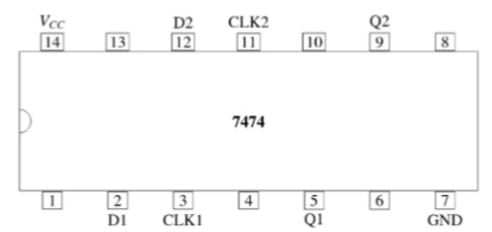
\includegraphics[width=0.35\textwidth]{Fig2}
\caption{\label{fig:Gates}}
\end{figure}
 \begin{table} [htbp]
\centering
\begin{tabular}{| c | c | c |} \hline
Components & Value & Quantity \\\hline
IC & 7474 & 1 \\ \hline
LEDs &  & 1 \\ \hline
Arduino & UNO & 1 \\ \hline
Jumper Wires &  & 10 \\ \hline
Breadboard & & 1 \\ 
\hline
\end{tabular}
\vspace{0.1cm}
\caption{\label{tab:widgets}}
\end{table}
\section{PROCEDURE}
\begin{enumerate}
	 \item Connect the Led's to the Arduino uno.
	 \item Give the inputs manually using jumper wires.
	 \item Truth Table for NAND and NOR gates.
		 \begin{table}[htbp]
			 \centering
			 \begin{tabular}{|c|c|c|c|}
				 \hline
				 A & B & A NOR B & A NAND B \\
				 \hline
				 0 & 0 & 1 & 1 \\
				 \hline
				 0 & 1 & 0 & 1 \\
				 \hline
				 1 & 0 & 0 & 1 \\
				 \hline
				 1 & 1 & 0 & 0 \\
				 \hline
			 \end{tabular}
			 \vspace{0.1cm}
			 \caption{\label{tab:widgets}}
		 \end{table}
	 \item Check the outputs by changing inputs as per truth table.
	 \item Execute the arduino code using the pio run command in nvim editor.
	 \item After upload the code into hardware setup using arduino IDE platform.
 \end{enumerate}
 \section{RESULT}
 Download the cod given in the link below and execute them to see the output as shown in Fig.2 by placing the LED at the output pin of 7474 IC. 
https://github.com/rajib05ra/FWC-Assignments/tree/main/Assignment%20IDE/IDE%20Code%20run/src
\begin{figure}[h] 
	\centering 
	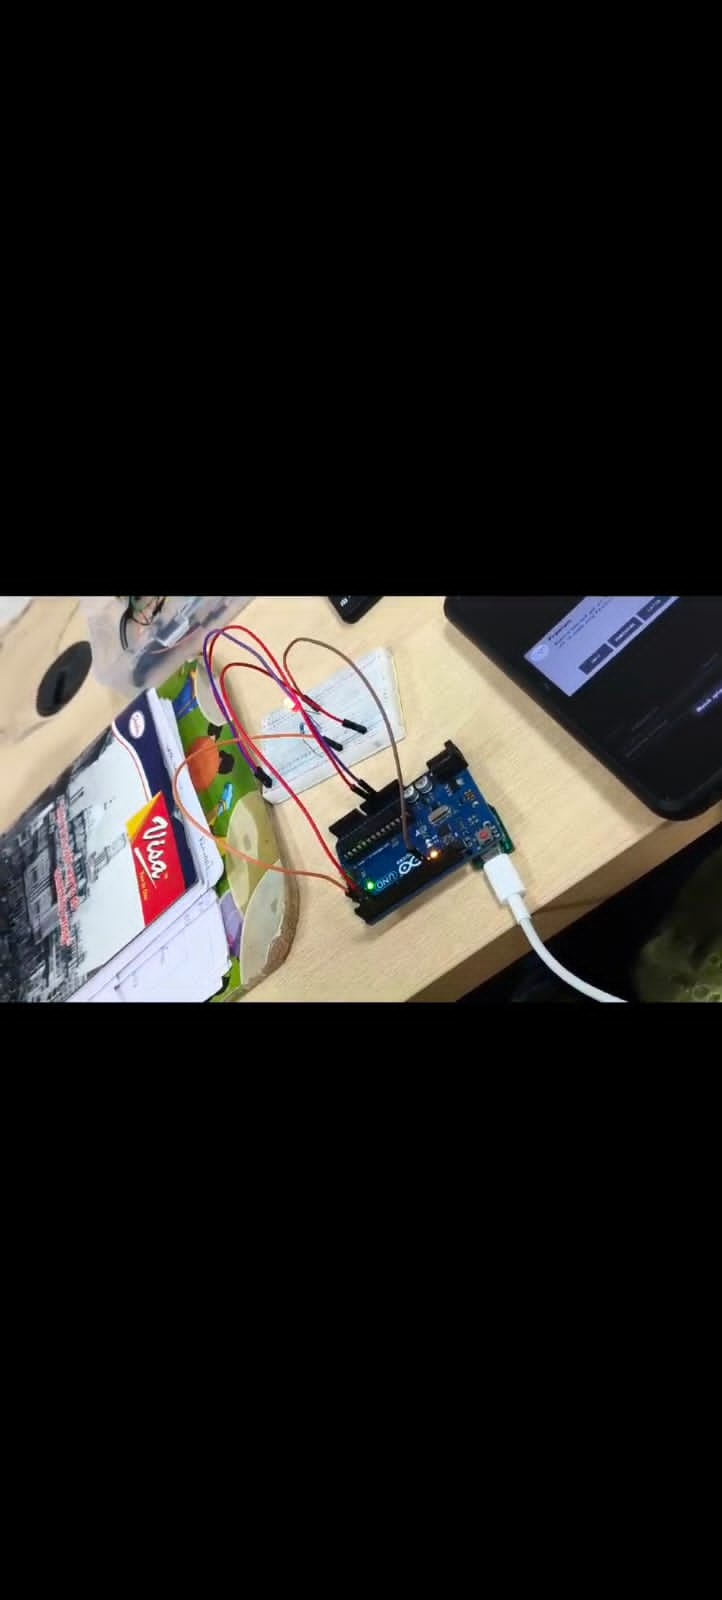
\includegraphics[width=0.35\textwidth]{Fig3}
	\caption{\label{fig:Gates}}    
\end{figure}
\section{CONCLUSION}
The D-Flip Flop is a good application in order to use it for registers. Here, the sequential circuit is combined with the combinational circuit of XOR gates to get the output. Therefore, we can design several circuits and can be implemented using Arduino and Platformio.
\end{document}

